\newcommand{\fwb}{1.6cm}  % width
\newcommand{\fwh}{1.2cm}     % height
\begin{figure}
\centering
\begin{tabular}{m{\fwb}m{2\fwb}}
%kernel & draws from GP & GP posterior \\
\rotatebox{90}{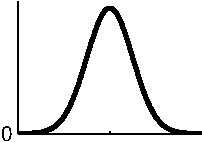
\includegraphics[width=\fwh,height=\fwb]{../figures/structure_examples/se_kernel}} 
& $\kernel_\textrm{SE}(\inputVar, \inputVar') = \sigma^2 \exp{\left(-\frac{(\inputVar - \inputVar')^2}{2\ell^2}\right)}$ \\
\rotatebox{90}{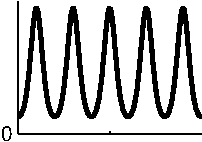
\includegraphics[width=\fwh,height=\fwb]{../figures/structure_examples/per_kernel}} 
& $\kernel_\textrm{Per}(\inputVar, \inputVar') = \sigma^2 \exp{\left(\frac{-2}{\ell^2}\sin^2(\frac{\pi|\inputVar - \inputVar'|}{p})\right)}$ \\
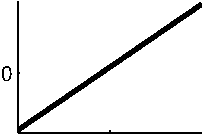
\includegraphics[width=\fwb,height=\fwh]{../figures/structure_examples/lin_kernel} 
& $\kernel_\textrm{Lin}(\inputVar, \inputVar') = \sigma_b^2 + \sigma_v^2(\inputVar - \ell)(\inputVar' - \ell)$
\end{tabular}
\caption{ Definitions of base kernels.  Left: a plot of each kernel as a function of one of its inputs.}
\label{fig:basic_kernels}
\end{figure}
